
\begin{figure}[h]
\centering
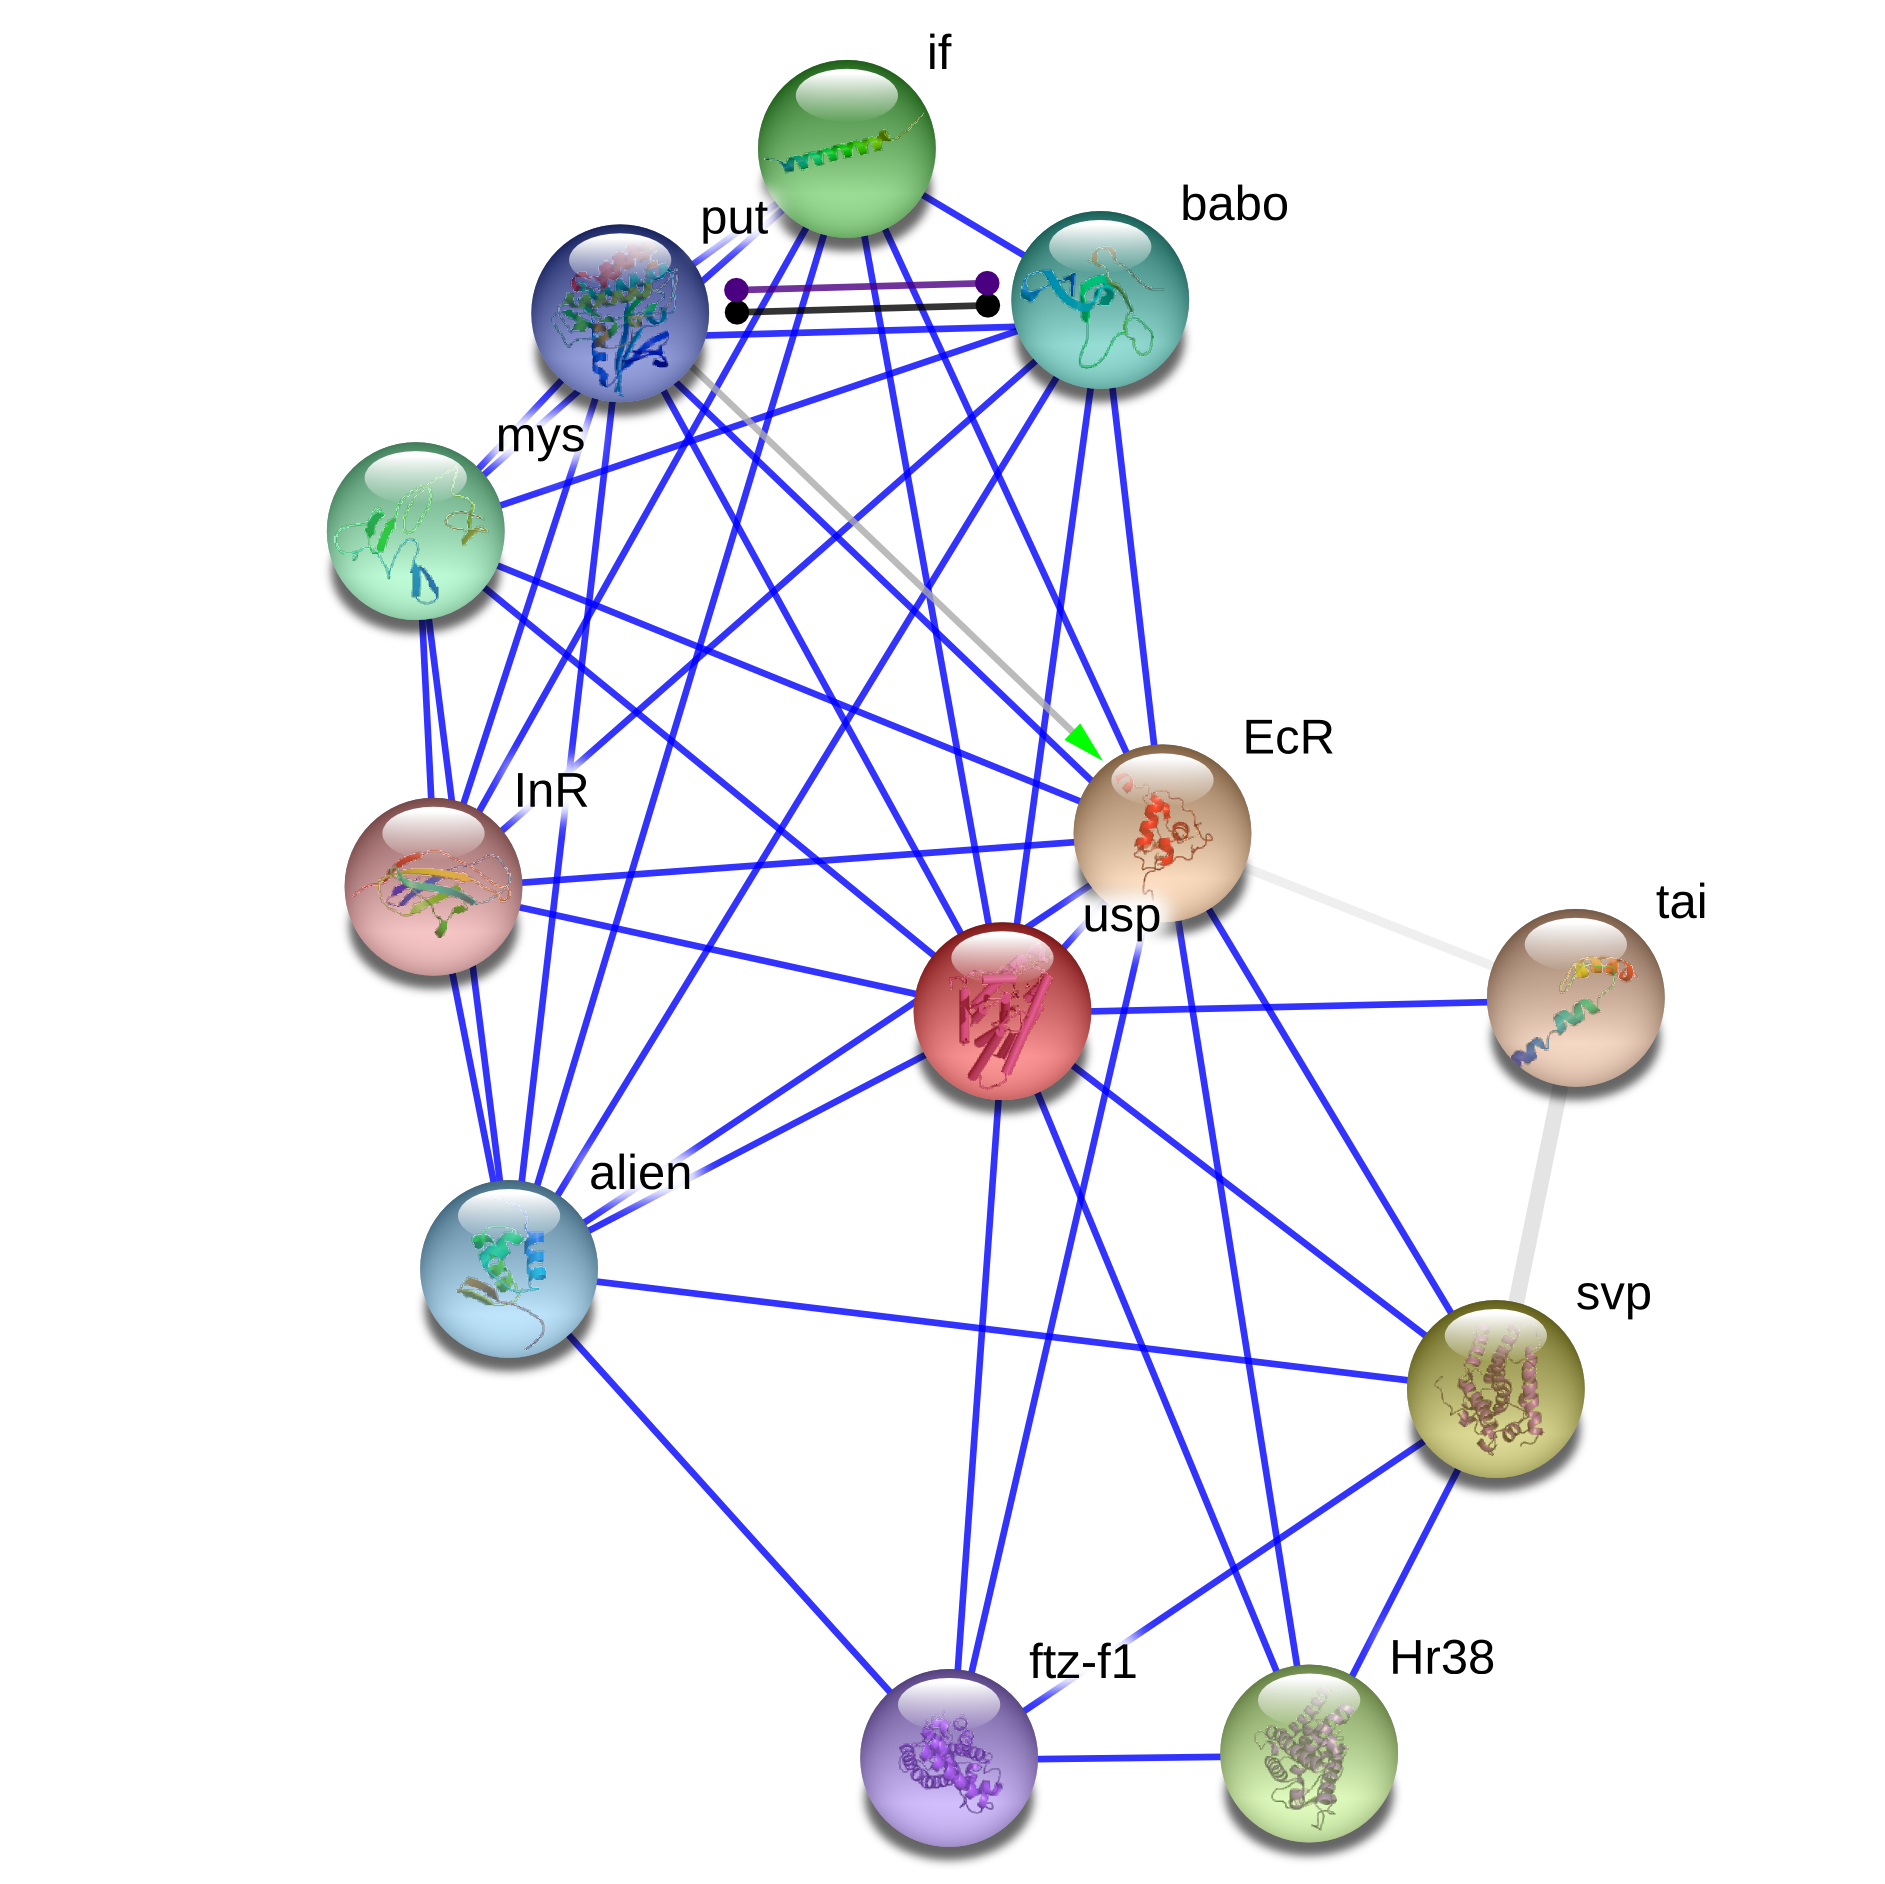
\includegraphics[width=.6\textwidth]{figures/figs/EcRUSP_graph.png}

\caption[Graphs are natural representations of biological relationships]{\sf \textbf{Graphs are natural representations of biological relationships.} Nodes (circles) represent proteins.
Edges (lines between nodes) represent interactions between nodes.
In a database scenario, edges and nodes can store multiple kinds of data in the form of key-value pair dictionaries (Figure \ref{fig:nway-ortholog-graph}) instead of a series of data tables grouped by a predefined schema as in relational databases.
}
\label{fig:ecrusp-graph}
\end{figure}